Tas ko sauc par ķēdi plašākā sabiedrībā tik stipri atšķirās no Bitcoin tehniskā apraksta\cite{nakamoto08} dotās definīcijas, ka tā vairs nav izmantojama. 
Lielākoties par ķēdi tiek saukta decentralizēta norēķinu sistēma, tomēr pa virsu šīm norēķinu sistēmām tiek veidoti arī citi servisi, kuriem ar naudas pārskaitījumiem nav nekāda sakara, piemēram domēna vārdu reģistra, sertefikātu autoritātes, vēlēšanu un citi servisi.\cite{namecoin} Arī šīs tiek sauktas par ķēdēm.
Turklāt esošās ķēžu implementācijas ir tik daudzveidīgas un ar atšķirīgu funkcionalitāti, ka ir grūti spriest kādās ir vispārīgas ķēdes īpašības.
Šajā nodaļā aplūkosim ar ķēdēm saistītas tēmas \textemdash{} decentralizētas sistēmas, digitālas valūtas un blokķēdē izmantotās datu struktūras. Beigās tiks aplūkotas konkrētas ķēdes realizācijas.

\subsection{Digitāla valūta}
Naudas atkārtota iztērēšana (double spending) ir kritiskākā digitālu valūtu problēma, kas ir analoģiska fiziskas naudas viltošanai, bet tā kā digitāla valūta pēc savas būtības glabājas uz datora, tad to ir viegli nokopēt neskaitāmos eksemplāros. Vienīgais veids, kā novērst problēmu ir, ja pārdevējs nelaiž pircēju ārā no veikala kamēr nav saņēmis apstiprinājumu par naudas īpašnieka maiņu no vienota patiesības avota.\cite{frankel96}

Mūsdienās par patiesības avotu parasti kalpo kāda centrāla organizācija, piemēram Visa vai PayPal, tomēr vienots patiesības avots var būt arī jebkurš izkliedētas sistēmas dalībnieks, ja visi tās dalībnieki laika gaitā pieņems vienādu stāvokli.
Ar parakstītu ziņojumu palīdzību ir iespējams izveidot autorizētus maksājuma pieprasījumus un šeit nav būtiskas atšķirības starp centralizētu un decentralizētu risinājumu. Savukārt sistēmai saņemot divus pieprasījumus no kuriem katrs atsevišķi ir derīgs, bet abi kopā izpildīties nevar, ir jāpieņem lēmums par to kurš izpildās un kurš ne.

Centralizētās sistēmās hronoloģiski pirmais pieprasījums tiktu izpildīts, bet vēlākais tiktu atteikts. Diemžēl decentralizētā gadījumā nav objektīva secība kurā pienāk ziņojumi. Ir nepieciešams vienprātības (consensus) algoritms, kas garantēs, ka visi maksājuma pieprasījumi tiek sakārtoti vienādā secībā visiem dalībniekiem, nodrošinot arī vienādu virsgrāmatas stāvokli.
Turklāt algoritmam jābūt noturīgam pret cenzūru un sabotāžu, lai tas būtu lietojams decentralizētā vidē.

\subsection{Datu struktūras}
Šajā nodaļā aplūkosim datu struktūras, kas ļauj pārliecināties par datu integritāti. Pieņemsim, ka ir nepieciešams iegūt lielu datu apjomu un ir uzticams avots no kura iegūt hash vērtību pret kuru var pārbaudīt, ka dati nav mainīti. 

Naivais veids būtu aprēķināt hash no visiem datiem un salīdzināt pret uzticamā avota sniegto hash vērtību. Problēma šādā pieejā ir tāda, ka iegūstot nedaudz atšķirīgus datus tie visi ir jāizmet un jāmeklē cits datu ieguves avots. Aplūkosim metodi, kas optimizē nepieciešamo komunikācijas daudzumu un dod iespēju iegūt datus no dažādiem avotiem vienlaicīgi.

Sadalīsim datus vairākās daļās un katrai daļai aprēķināsim hash vērtību. Tad sarēķina hash no visām iepriekš iegūtajām hash vērtībām un šo izmanto par galveno (saknes) hash vērtību, kas iegūta no uzticamā avota.\ref{fig:hash-list} 

\begin{figure}[htpb]
    \centering
    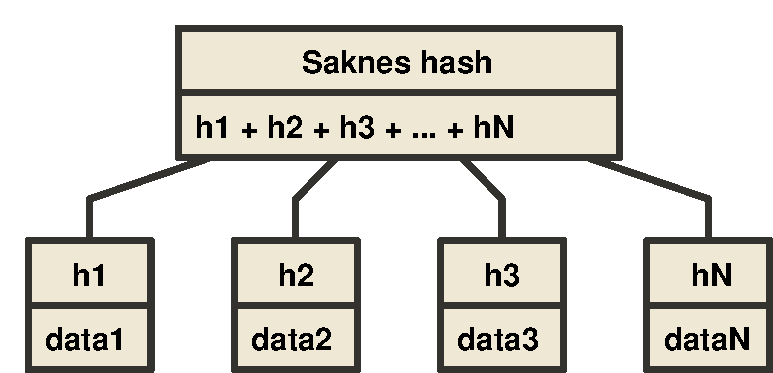
\includegraphics[scale=0.5]{teorija/hash-list.pdf}
    \caption{Hash saraksts}
    Dati tiek sadalīti vairākās daļās katrai daļai tiek aprēķināta hash vērtība. Saknes hash tiek aprēķināts no atsevišķo daļu hash vērtībām.
\label{fig:hash-list}
\end{figure}

Tagad pirms sākt datu ieguvi tiek iegūts saraksts ar hash vērtībām sadalītajiem datiem. Ievēro, ka informācijas apjoms, kas jāpārsūta šajā gadījumā ir ievērojami mazāks par visu datu apjomu. Sarēķina vai hash no saraksta atbilst tam kas tiek iegūts no drošā avota, ja rodas nesakritība, tad ir skaidrs, ka nav vērts sākt pašu datu lejuplādi. Kad ir veiksmīgi iegūts pareizais hash saraksts, tad lejuplādi datiem var veikt no vairākiem avotiem prasot katram avotam savus datu gabaliņus, kā arī uzreiz izķert kļūdas.

Līdzīgi mehānismi tiek izmantoti decentralizētos failu apmaiņas protokolos piemēram BitTorrent. Metode strādā ļoti labi, ja dati laika gaitā ir nemainīgi, tomēr mainīgiem datiem būtu neparocīgi katru reizi pārrēķināt galveno hash vērtību, jo tad tā ir jāmaina uzticamajam avotam. Aplūkosim metodi, kas ļauj ar nemainīgu galveno hash vērtību validēt datus, kuri regulāri tiek pagarināti, bet vēsture paliek nemainīga.

Aplūkojamā datu struktūra sastāv no blokiem, kuri paši sastāv no datiem un iepriekšējā bloka hash vērtības. Pats pirmais bloks, kas satur sākotnējo vērtību, nesatur sevī hash vērtību un šo bloku sauc arī par \textit{genesis block}. Datu struktūra ir līdzīga saistītajam sarakstam, bet atšķirība ir tāda, ka nav iespējams mainīt bloka saturu, vai ievietot pa vidu vēl kādu bloku.\ref{fig:hash-chain}

\begin{figure}[htpb]
    \centering
    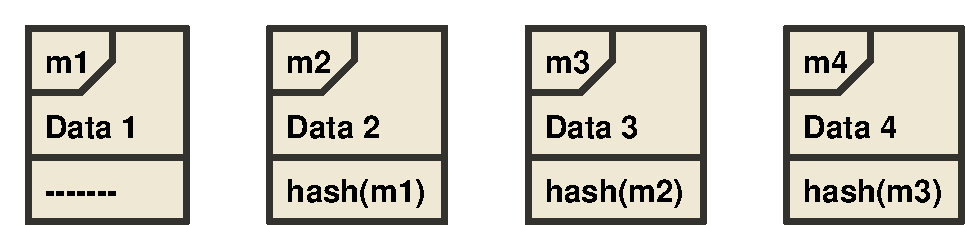
\includegraphics[scale=0.5]{teorija/hash-chain.pdf}
    \caption{Hash ķēde}
    Katrs hash ķēdes ziņojums $m_i$ sastāv no sev raksturīgajiem datiem $d_i$ un
    iepriekšējā posma $m_{i-1}$ hash vērtības.
\label{fig:hash-chain}
\end{figure}

Piemēram, pamainot otrā bloka datu vērtību mainās bloka hash un tas vairs nesakrīt ar trešajā blokā ierakstīto hash vērtību. Savukārt izmainot trešajā blokā ierakstīto otrā bloka hash vērtību izmainās trešā bloka hash, salaužot ceturto bloku. Tātad, lai izmainītu datus blokā $i$ ir jāizmaina visi bloki, kuri seko $i$.

\subsection{Izkliedētā skaitļošana (distributed computing)}
Aprakstīsim Bizantijas vienošanās problēmu (Byzantine agreement, Byzantine generals problem).
Pieņemsim, ka ir sistēma kas sastāv no tīklā saslēgtiem datoriem, kuri sazinās savā starpā sūtot ziņojumus. Mērķis ir vienoties par koordinētu tālāko rīcību, kas ir atkarīga no ārējiem apstākļiem, kuri iepriekš nav zināmi. Uzdevumu padara grūtu tas, ka starp datoriem var būt arī tādi, kas ļaunprātīgi cenšas sabotēt vienotu rīcību.
Problēmas atrisinājums ir vienprātības algoritms, kuram izpildās divas īpašības.
\begin{enumerate}
    \item Datoram izpildot algoritmu tiek pieņemts tāds pats lēmums, kā citiem datoriem, kuri izpilta algoritmu.
    \item Neliels daudzums ar ļaunprātīgiem datoriem nespēj ietekmēt pieņemto lēmumu.
\end{enumerate}\cite{lamport82}
Turpmāk datoru šīs problēmas kontekstā sauksim par \textbf{virsoni} (node), jo tie ir tīklā saslēgti vienlīdzīgi elementi. Veiksim arī citas nelielas modifikācijas
Pēc katra pieņemtā lēmuma tīkla stāvoklis būs mainījies un lēmuma pieņemšanu būs nepieciešams atkārtot. Teiksim ka katram pieņemtajam lēmumam $x$ ir indekss $i$. Virsotne var droši \textbf{publicēt} vērtību $x$ pozīcijā $i$, ja visiem iepriekšējiem indeksiem ir publicēts kāds lēmums un virsotne ir pārliecināta, ka arī citas virsotnes laika gaitā publicēs vērtību $x$ pozīcijā $i$.\cite{mazieres15} Tādējādi mēs neprasām, lai visas virsotnes pieņemtu vienotu lēmumu vienlaicīgi, bet gan to, lai vienots lēmums eksistētu. Šāda modifikācija noteikti ir nepieciešama, jo decentralizētā vidē nav pat zināms dalībnieku skaits.
Pieņemtais lēmums mūsu gadījumā virsgrāmata.

Tā kā darbojamies decentralizētā vidē, tad viens ļaundaris bez problēmām var izlikties par vairākām virsotnēm vienlaicīgi. Tādēļ otro nosacījumu padarīsim spēcīgāku un skaidrāku, prasot, lai jebkāds daudzums ar ļaunprātīgām virsotnēm nespēj ietekmēt pieņemto lēmumu.
Kļūst skaidrs, ka mūsu gadījumā demokrātiska lēmuma pieņemšana nav risinājums, tapēc aplūkosim populārākos līdz šim piedāvātos vienprātības algoritmus.
% proof of work
% proof of stake
% fba
% proof of ddos

\subsubsection{Pierādījums ar darbu (Proof of work)}
\subsubsection{Pierādījums ar risku (Proof of stake)}
\subsubsection{Federatīva Bizantijas vienošanās (FBA)}
Papildināsim uzdevumu ar sekojošajām definīcijām.
Virsotņu kopu sauc par \textbf{drošu}, ja katrām divām virsotnēm tās publicēs vienādas vērtības.
Virsotni sauc par \textbf{dzīvu}, ja spēj publicēt jaunas vērtības nepaļaujoties uz ļaunprātīgo virsotņu sadarbību.
Virsotņu kopu sauc par \textbf{pareizu}, ja tā ir droša un katra virsotne ir dzīva.
\subsubsection{Pierādījums ar DDoS (Proof of DDoS)}
% ielikt no stellar whitepaper bildi 7lpp

% Protokolam jāpanāk, ka visas ļaunprātīgās virsotnes laika gaitā publicēs tās pašas izmaiņas.

% Failu apmaiņa starp vienaudžiem (p2p), izmantojot BitTorrent protokolu, ir pierādījusi sevi kā praktiski necenzējamu sistēmu. Ja kāds fails tīklā kļūst populārs, tad ir pamats ticēt, ka tas nevar no turienes pazust. Veiksmīgākie mēģinājumi cīnīties pret dalīšanos BitTorrent tīklā ir saistīti ar uzbrukumiem tādiem serveriem, kas uztur sarakstu ar tīklā atrodamajiem failiem. Tomēr ir ieviesti strādājoši paplašinājumi BitTorrent protokolam, kas ļauj atrast failus decentralizētā vidē un iepriekšminētie serveri vairs nav nepieciešami.\cite{pouwelse08}


% \begin{description}
%     \item[Decentralizētas sistēmas] Torenti, Bizantijas ģenerāļu problēma, vienprātības nepieciešamība sakārtotas vēstures uzturēšanai.
%         % torrenti, BGP, consensus nepieciešamība, anti spam nepieciešamība <- parakstu nepieciešamība
%         \item[Digitālas valūtas]
%         % double spending, te kļūst skaidrs, ka secība ir svarīga.
%         % reusability
%         \item[Blokķēdes realizācijas]
%         % hash chain
%         %% skip list
%         %% merkle tree
%         % consensus algorithms
%         %% proof of work 
%         %% proof of stake
%         %% fba
%         %% proof of ddos
% \end{description}

% pameklēt fair exchange blockchain
% pameklēt blockchain abstraktu klasifikāciju iekš scholar
% ja neizdodas tad definēt: forumu, izdevniecību, tirgu, necenzētu

% viena no īpašībām ir spēja atrisināt Byzantine Generals Problem bet tas nav svarīgi šajā kontekstā
% kas ir DA0
